\begin{frame}{Reduced Basis Method}
	\Large{\highlightB{RB workflow}}
	\normalsize
	\vspace{5mm}
	\begin{figure}
		\tikzset{
	main/.style={black, line width=0.4mm, opacity=1},
	second/.style={gray, opacity=5},
	arrow/.style={-latex, shorten >=1ex, shorten <=1ex, bend angle=45}
}
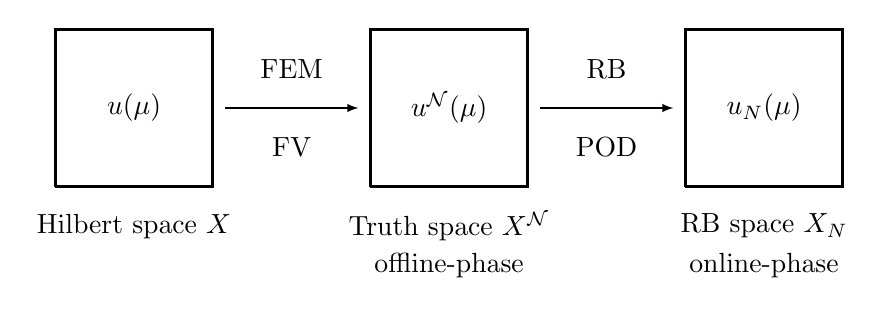
\begin{tikzpicture}
%% Global Matrix
\draw[main] (0,0) -- (2,0) -- (2,2)-- (0,2)-- (0,0);
\draw[main] (4,0) -- (6,0) -- (6,2)-- (4,2)-- (4,0);
\draw[main] (8,0) -- (10,0) -- (10,2)-- (8,2)-- (8,0);


\draw [arrow]  (2,1) to (4,1);
\draw [arrow]  (6,1) to (8,1);


\draw (1,1) node {$u(\mu)$};
\draw (5,1) node {$u^\mathcal{ N }(\mu)$};
\draw (9,1) node {$u_N(\mu)$};

\draw (3,1.5) node {FEM};
\draw (3,.5) node {FV};

\draw (7,1.5) node {RB};
\draw (7,.5) node {POD};

\draw (1,-.5) node {Hilbert space $\mathbb{X}$};
\draw (5,-.5) node {Truth space $\mathbb{X}^\mathcal{ N }$};
\draw (5,-1) node {offline-phase};
\draw (9,-.5) node {RB space $\mathbb{X}_N$};
\draw (9,-1) node {online-phase};


\end{tikzpicture} 
	\end{figure}

	\begin{align*}
	\text{find }u(\mu) \in \mathbb{X} :\quad a(u(\mu),v;\mu) = f(v;\mu) \quad \forall v \in \mathbb{X}.
	\end{align*}
		
\end{frame}

\begin{frame}{Reduced Basis Method}
	\Large{\highlightB{Truth problem}}
	\normalsize
	\begin{align*}
	\text{find }u^\mathcal{ N }(\mu) \in \mathbb{X^\mathcal{ N }} :\quad a(u^\mathcal{ N }(\mu),v;\mu) = f(v;\mu) \quad \forall v \in \mathbb{X^\mathcal{ N }}.
	\end{align*}
	\Large{\highlightB{Truth solutions}}
	\begin{align*}
	u^\mathcal{ N }(\mu) = \sum_{i=1}^{\mathcal{ N }} u_{i}^\mathcal{ N }(\mu) \cdot \varphi_i,  \quad   \mathbb{X^\mathcal{ N }} = \text{span}(\varphi_1, ...,  \varphi_\mathcal{ N })
	\end{align*}
	\Large{\highlightB{Goal: Approximate solution manifold}}\\
	\begin{align*}
	\mathbb{M^\mathcal{N}} = \{u^\mathcal{N}(\mu),\quad \mu \in \mathbb{P}\}
	\end{align*}
	
\end{frame}

\begin{frame}{Reduced Basis Method}
	\Large{\highlightB{Reduced Space}}
	
	\begin{align*}
	\mathbb{X}_N = \text{span}(\xi_1, ..., \xi_N), \qquad N \ll \mathcal{ N } 
	\end{align*}
	\Large{\highlightB{Reduced solutions}}
	\begin{align*}
	u_N (\mu) = \sum_{i=1}^{ N } u_{N,i}(\mu) \cdot \xi_i
	\end{align*}
	
	\Large{\highlightB{Reduced problem}}
	\normalsize
	\vspace{0.5cm}
	\begin{align*}
	\text{find }u_N(\mu) \in \mathbb{X}_N :\quad a(u_N(\mu),v;\mu) = f(v;\mu) \quad \forall v \in \mathbb{X}_N
	\end{align*}
	
	
\end{frame}

